\chapter{}

\textbf{\underline{Problem text}:} Define the temperature dependence of the potential (interactive) energy of water molecules in 1 kg of water.

\textbf{\underline{Solution}:} Let's choose the zero potential energy level corresponding to the potential energy of steam at its boiling temperature $T_\text{v}=373$ K. Then, as the kinetic energy of a single molecule in liquid water and steam is the same and equal to $3kT_\text{v}$ ($k$ is the Boltzmann constant), the potential energy of water at its boiling temperature is equal to $W(T_\text{v})=-L$ per unit mass (here $L=2,\hspace{-1.3pt}26\cdot 10^6$ J/kg is the latent heat of vaporization).

To calculate the temperature dependence of the potential energy, a list of values of heat capacity of water at different temperatures is needed. As a good approximation, the heat capacity of water can be considered constant and equal to $c_\text{w}=4,\hspace{-1.3pt}19\cdot 10^3$ J/(kg\,$\cdot$\,K). As the full energy is equal to the sum of the kinetic and the potential energies, and its change is proportional to the heat capacity of water, then the potential energy (per unit mass) depends on the temperature as
$$
  W(T)=W(T_\text{v})-c_\text{w}\left(T_\text{w}-T\right)+\frac{3R\left(T_\text{w}-T\right)}{\mu}=-L-c_\text{w}\left(T_\text{w}-T\right)+\frac{3R\left(T_\text{w}-T\right)}{\mu},
$$
where $R=8,\hspace{-1.3pt}314$ J/(mol\,$\cdot$\,K) is the universal gas constant, $\mu=18,\hspace{-1.3pt}0$ g/mol is the molar mass of water. A graph $W(T)$ was plotted according to this formula (see fig. \ref{energy})

For a more precise calculation the temperature dependence of the heat capacity of water is required. The corresponding table is given below\footnote{\href{http://www.engineeringtoolbox.com/water-thermal-properties-d_162.html}{Source link}}.

\begin{center}
\begin{tabular}{|c|c|c|c|c|c|c|c|c|c|c|c|c|}
\hline
$T$, \degree C & 0,01 & 5 & 10 & 15 & 20 & 25 & 30 & 35 & 40 & 45 & 50\\
\hline
$c_\text{w}$, J/(kg\,$\cdot$\,K) & 4,210 & 4,204 & 4,193 & 4,1855 & 4,183 & 4,181 & 4,179 & 4,178 & 4,179 & 4,181 & 4,182\\
\hline
$T$, \degree C & 55 & 60 & 65 & 70 & 75 & 80 & 85 & 90 & 95 & 100 &\\
\hline
$c_\text{w}$, J/(kg\,$\cdot$\,K) & 4,183 & 4,185 & 4,188 & 4,191 & 4,194 & 4,198 & 4,203 & 4,208 & 4,213 & 4,219 &\\
\hline
\end{tabular}
\end{center}

\begin{wrapfigure}{r}{195pt}
\begin{center}
\vspace{-4mm}
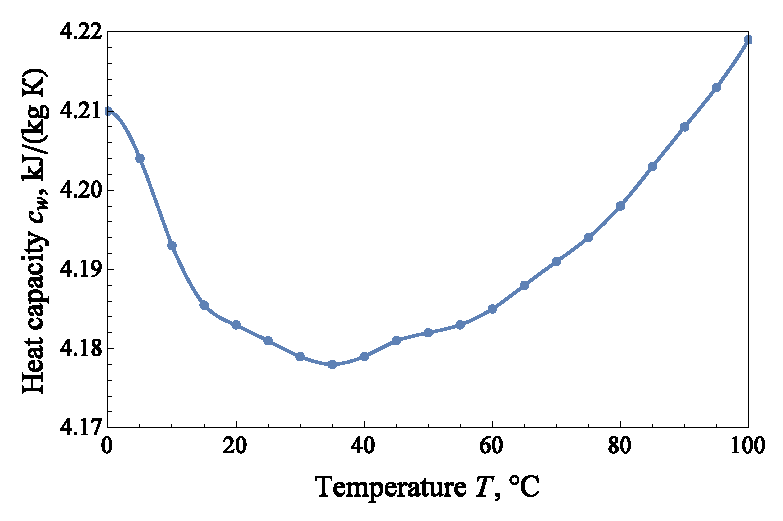
\includegraphics[scale=0.55]{1/fig12eng.eps}
\end{center}
\vspace{-2mm}
\caption{the temperature dependence of the heat capacity of water.}\label{heatcapacity}
\end{wrapfigure}

A graph is plotted due to the given table (see fig. \ref{heatcapacity}). Then an interpolational curve is fit through the given points with the program \textit{Mathematica}\footnote{The full name of the program is \textit{Wolfram Mathematica}, see \href{http://www.wolfram.com/mathematica/}{here}}, it is also shown in fig. \ref{heatcapacity}. Using this curve as the function $c_\text{w}(T)$, the temperature dependence of the potential energy of water can be expressed as
$$
  W(T)=-L-\int\limits_T^{T_\text{v}} c_\text{w}(T)dT+\frac{3R\left(T_\text{w}-T\right)}{\mu}.
$$

This dependence can be easily calculated using numerical integration, the corresponding graph is given on fig. \ref{energy}. For comparison, a difference graph $\Delta W(T)$ is plotted below (see fig. \ref{difenergy}), in which the heat capacity for the first method is taken to be the average on the graph (see fig. \ref{heatcapacity}) for zeroing the values at the interval ends (the precise value is $c_\text{w}=4,\hspace{-1.3pt}1911$ kJ/(kg\,$\cdot$\,K)).

\textbf{\underline{Answer}:} see graphs.

\begin{figure}[!h]
\begin{center}
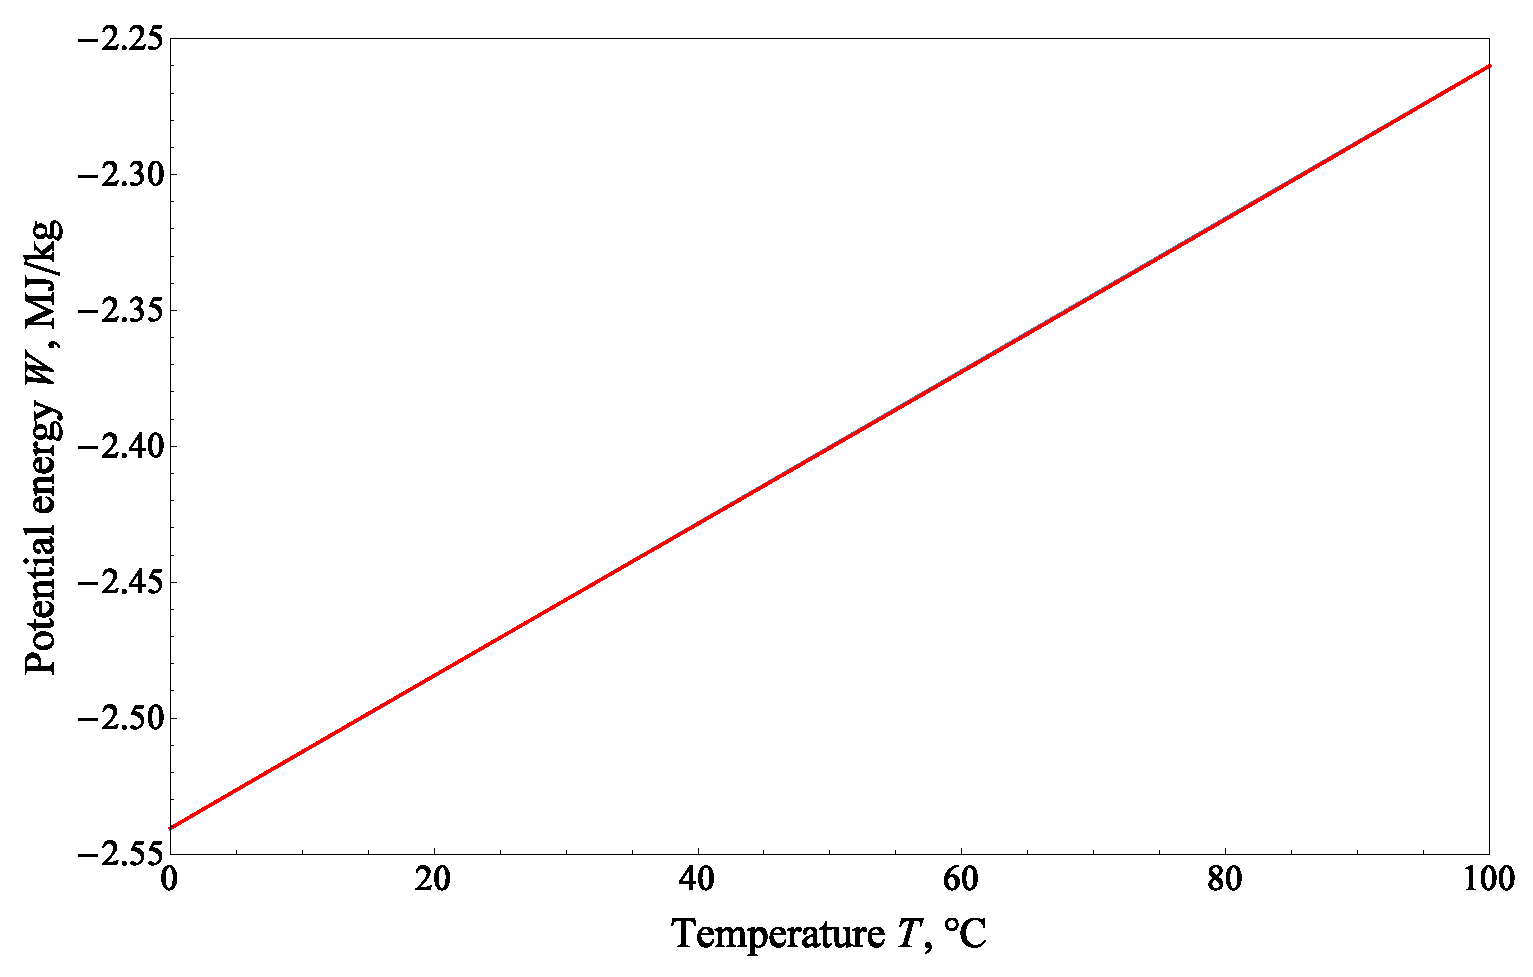
\includegraphics[scale=0.65]{1/fig13eng.eps}
\end{center}
\caption{the temperature dependence of the potential energy of water. The graph from the second method is colored red, the graph from the first method is blue (merges with the red one on the figure).}\label{energy}
\end{figure}

\begin{figure}[!h]
\begin{center}
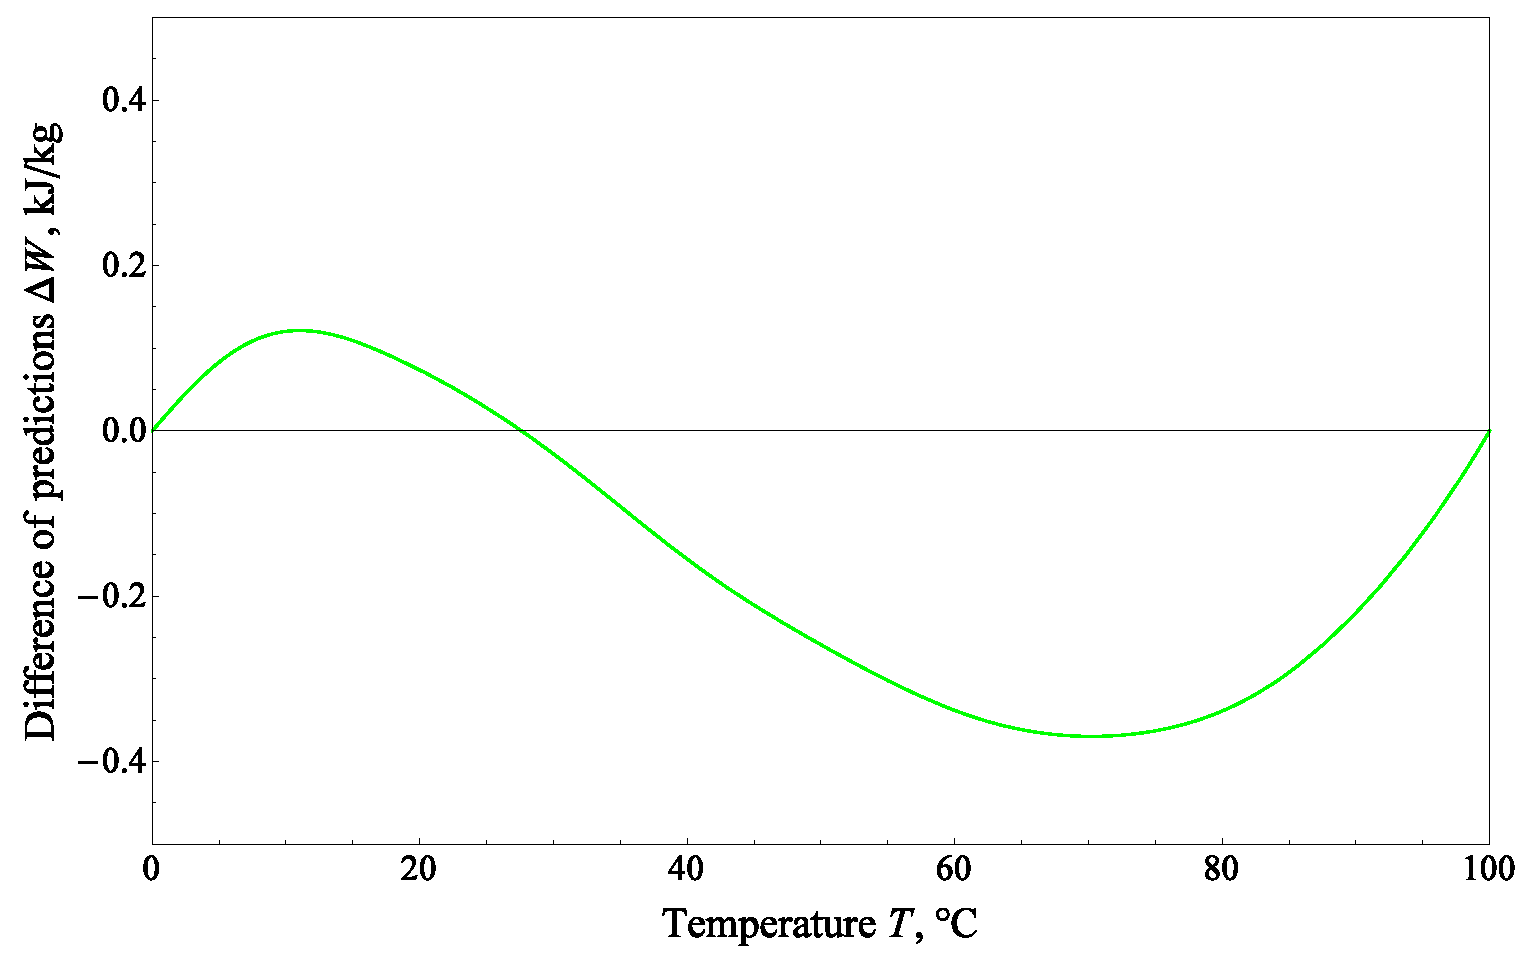
\includegraphics[scale=0.65]{1/fig14eng.eps}
\end{center}
\caption{the difference graph of the two dependencies above. Pay attention at the scale on the axis (kJ/kg)!}\label{difenergy}
\end{figure} 